\documentclass[tikz,border=8pt]{standalone}
\usepackage{amsmath}
\usetikzlibrary{positioning, arrows.meta, calc}

\begin{document}

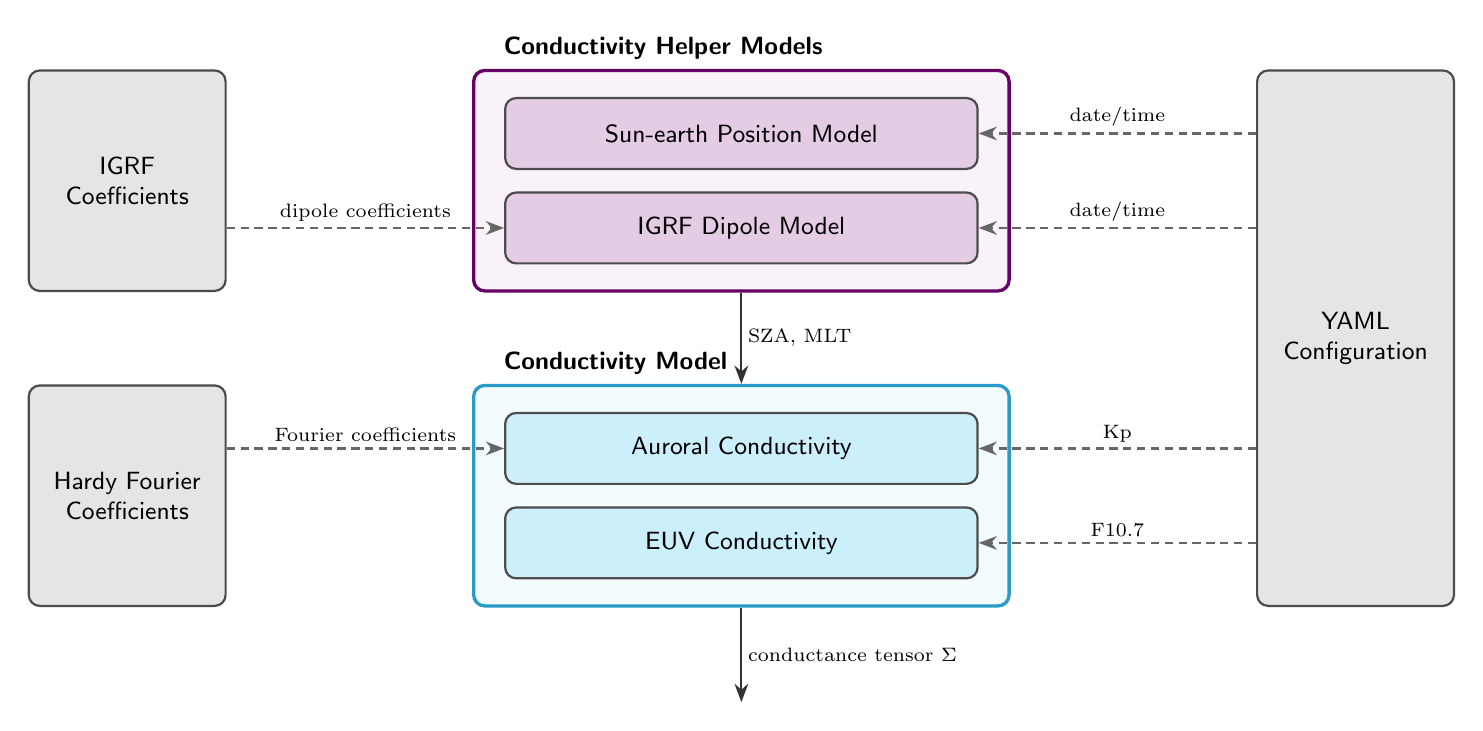
\begin{tikzpicture}[
		>=Stealth,
		% Standard composite box style (fixed size to ensure exact stacking)
		compbox/.style 2 args={
				rectangle, rounded corners, draw=#1!80!black, very thick,
				fill=#1!5, minimum width=6.8cm, minimum height=2.8cm,
				label={[anchor=south west, font=\sffamily\small\bfseries, xshift=8pt, yshift=0pt]north west:#2}
			},
		% Inner sub-boxes
		subbox/.style={
				rectangle, rounded corners, draw=black!70, thick,
				fill=#1!20, minimum width=6.0cm, minimum height=0.9cm,
				font=\sffamily\small, align=center
			},
		% Standard standalone blocks
		stdbox/.style={
				rectangle, rounded corners, draw=black!70, thick,
				fill=#1!20, font=\sffamily\small, align=center
			},
		% Arrows
		arrowdata/.style={->, thick, draw=black!80},
		arrowparam/.style={->, densely dashed, thick, draw=black!60},
		labarrow/.style={font=\scriptsize, fill=white, inner sep=2pt, align=center}
	]

	% ==========================================
	% 1. MAIN VERTICAL STACK (X=0)
	% ==========================================
	% All central blocks strictly share minimum width=6.8cm and height=2.8cm

	% Block 1: Helper Models (Y=0)
	\node[compbox={violet}{Conductivity Helper Models}] (helper) at (0, 0) {};
	\node[subbox=violet] (sunearth) at ([yshift=0.6cm]helper.center) {Sun-earth Position Model};
	\node[subbox=violet] (igrf) at ([yshift=-0.6cm]helper.center) {IGRF Dipole Model};

	% Block 2: Conductivity Model (Y=-4.0)
	\node[compbox={cyan}{Conductivity Model}] (cond) at (0, -4.0) {};
	\node[subbox=cyan] (auroral) at ([yshift=0.6cm]cond.center) {Auroral Conductivity};
	\node[subbox=cyan] (euv) at ([yshift=-0.6cm]cond.center) {EUV Conductivity};


	% ==========================================
	% 2. EXTERNAL DATA SOURCES (LEFT, X=-7.8)
	% ==========================================

	% New Data Box 1: IGRF Coefficients (Aligned with Helper Models at Y=0)
	\node[stdbox=gray, minimum width=2.5cm, minimum height=2.8cm]
	(igrfcoef) at (-7.8, 0.0) {IGRF\\Coefficients};

	% New Data Box 2: Hardy Fourier Coefficients (Aligned with Conductivity Model at Y=-4.0)
	\node[stdbox=gray, minimum width=2.5cm, minimum height=2.8cm]
	(hardycoef) at (-7.8, -4.0) {Hardy Fourier\\Coefficients};


	% ==========================================
	% 3. YAML CONFIGURATION (RIGHT, X=7.8)
	% ==========================================
	% Width = 2.5cm, pushed out to X=7.8 to increase gap
	% Height adjusted to 6.8cm to match the shorter stack.

	\node[stdbox=gray, minimum width=2.5cm, minimum height=6.8cm]
	(yaml) at (7.8, -2.0) {YAML\\Configuration};


	% ==========================================
	% 4. DATA FLOW ARROWS (SOLID)
	% ==========================================

	% Vertical pipeline data flow (Length is exactly 1.2cm)
	\draw[arrowdata] (helper.south) -- node[labarrow, right] {SZA, MLT} (cond.north);

	% Final data output arrow pointing to the bottom
	% Node is placed midway to precisely match the positioning of the arrow above
	\draw[arrowdata] (cond.south) -- node[labarrow, right] {conductance tensor $\Sigma$} ++(0,-1.2);


	% ==========================================
	% 5. PARAMETER FLOW ARROWS (DASHED)
	% ==========================================

	% From Left Data Boxes into Sub-models
	\draw[arrowparam] (igrfcoef.east |- igrf.west) -- node[labarrow, above] {dipole coefficients} (igrf.west);
	\draw[arrowparam] (hardycoef.east |- auroral.west) -- node[labarrow, above] {Fourier coefficients} (auroral.west);

	% From YAML into Helper sub-boxes
	\draw[arrowparam] (yaml.west |- sunearth.east) -- node[labarrow, above] {date/time} (sunearth.east);
	\draw[arrowparam] (yaml.west |- igrf.east) -- node[labarrow, above] {date/time} (igrf.east);

	% From YAML into Conductivity sub-boxes
	\draw[arrowparam] (yaml.west |- auroral.east) -- node[labarrow, above] {Kp} (auroral.east);
	\draw[arrowparam] (yaml.west |- euv.east) -- node[labarrow, above] {F10.7} (euv.east);

\end{tikzpicture}

\end{document}
